\section{Upgrading FX3 Firmware} \label{sec:fw-upgrade}

The firmware executing on the bladeRF's Cypress \fx3 USB peripheral controller
may be updated via a few different methods. Note that there are generally
dependencies between the firmware, the FPGA bitstream, and host software
versions. These dependencies are listed in the bladeRF \fname{CHANGELOG} file
and release notes.

\textit{``Don't Panic!''} It is generally \textbf{not} possible to ``brick'' or damage
the device by accidentally unplugging a device or by closing a program during a
firmware upgrade. In these cases, the \fx3 will enter a recovery bootloader
mode.  Furthermore, it is always possible to force the device into this
recovery state, as detailed in this section.

\subsection{Obtaining Firmware}
Official firmware releases may be obtained from the Nuand webiste: \\
\centerline{\url{https://nuand.com/fx3}}

The following URL always points to the latest available release: \\
\centerline{\url{https://nuand.com/fx3/bladeRF\_fw\_latest.img}}

The remainder of this section assumes the firmware file is named
\fname{bladeRF\_fw\_latest.img} and is located in the current working directory.
Be sure to adjust this accordingly for your specific firmware file and location.

\subsection{Upgrading Firmware via bladeRF-cli}

The \bladerfcli may be used to flash firmware from the command-line 
or in in its interactive mode.

The procedure is as follows:
\begin{enumerate}
    \item Flash new firmware via \bladerfcli.
    \item Power-cycle the device to boot new firmware.
    \item Note the new version number being reported by \bladerfcli.
\end{enumerate}

The commands show in \ref{sec:fw-upgrade-cli} or \ref{sec:fw-upgrade-interactive}
may be used.

\newpage
\subsubsection{Command-line} \label{sec:fw-upgrade-cli}
\begin{lstlisting}[style=numbered-snippet]
$ bladeRF-cli -f bladeRF_fw_latest.img
Flashing firmware...
[INFO @ usb.c:498] Erasing 3 blocks starting at block 0
[INFO @ usb.c:503] Erased block 2
[INFO @ usb.c:511] Done erasing 3 blocks
[INFO @ usb.c:705] Writing 464 pages starting at page 0
[INFO @ usb.c:709] Writing page 463
[INFO @ usb.c:718] Done writing 464 pages
[INFO @ flash.c:110] Verifying 464 pages, starting at page 0
[INFO @ usb.c:603] Reading 464 pages starting at page 0
[INFO @ usb.c:606] Reading page 463
[INFO @ usb.c:617] Done reading 464 pages
Done. A power cycle is required for this to take effect.

# Power cycle device here

$ bladeRF-cli -e version

  bladeRF-cli version:        1.3.1
  libbladeRF version:         1.5.1

  Firmware version:           1.9.0
  FPGA version:               0.5.0
\end{lstlisting}

\subsubsection{Interactive Mode} \label{sec:fw-upgrade-interactive}
\begin{lstlisting}[style=numbered-snippet]
$ bladeRF-cli -i
bladeRF> load fx3 bladeRF_fw_latest.img

  Flashing firmware from bladeRF_fw_latest.img...

[INFO @ usb.c:498] Erasing 3 blocks starting at block 0
[INFO @ usb.c:503] Erased block 2
[INFO @ usb.c:511] Done erasing 3 blocks
[INFO @ usb.c:705] Writing 464 pages starting at page 0
[INFO @ usb.c:709] Writing page 463
[INFO @ usb.c:718] Done writing 464 pages
[INFO @ flash.c:110] Verifying 464 pages, starting at page 0
[INFO @ usb.c:603] Reading 464 pages starting at page 0
[INFO @ usb.c:606] Reading page 463
[INFO @ usb.c:617] Done reading 464 pages
  Done. Cycle power on the device.

bladeRF> quit
$

# Power cycle device here

$ bladeRF-cli -i
bladeRF> version

  bladeRF-cli version:        1.3.1
  libbladeRF version:         1.5.1

  Firmware version:           1.9.0
  FPGA version:               0.5.0

bladeRF> quit
\end{lstlisting}

\newpage
\subsection{Recovering from the Bootloader} \label{sec:recovery}

The \fx3 on the bladeRF falls back to a USB bootloader mode if valid
firmware is not found in SPI flash. In this mode, the device enumerates
with a \texttt{VID:PID = 04b4:00f3}. 

The \cmd{recover} command in \bladerfcli may be used identify
devices in this bootloader state and download firmware to their RAM.

The general recovery procedure, outlined in the remainder of this section is:
\begin{enumerate}
    \item Identify device(s) in bootloader mode
    \item Download and boot firmware from RAM
    \item Write firmware to SPI flash
\end{enumerate}

\subsubsection{Detecting a Device in Bootloader Mode}
When starting up, \bladerfcli detects devices in this bootloader mode
and prints a message alerting users to this: \\

\begin{lstlisting}[style=snippet]
    NOTE: One or more FX3-based devices operating in bootloader mode
          were detected. Run 'help recover' to view information about
          downloading firmware to the device(s).

    No bladeRF device(s) available.
    
    If one is attached, ensure it is not in use by another program
    and that the current user has permission to access it.
\end{lstlisting}

The devices in bootloader mode may be printed using the \cmd{recover} command
with no arguments: \\

\begin{lstlisting}[style=snippet]
bladeRF> recover

  FX3 bootloader devices:
  ---------------------------------------------------------
    Backend:    libusb
    Bus:        1
    Address:    11

  Use 'recover <bus> <addr> <firmware>' to download and boot
  firmware to the specified device.
\end{lstlisting}

\textit{\textbf{Troubleshooting for \windows users}:}
If a device in bootloader mode is not detected, or \bladerfcli fails to open it
via the \cmd{recover} command, it may be the case that \windows is using driver
that is incompatible with \bladerfcli. In this case, one may use \program{Zadig}
 \cite{ZADIG} to install a libusb-compatible driver.

\subsubsection{Downloading Firmware to RAM}
Firmware may be downloaded to the USB peripheral controller's RAM as shown in the
following snippet.  The device will immediately begin executing this firmware,
allowing the device to be opened in \bladerfcli.

{
\noindent\minipage{\linewidth}\medskip
\begin{lstlisting}[style=numbered-snippet]

bladeRF> recover 1 11 bladeRF_fw_latest.img

  Success! Use "open" to switch to this device.
  Note that a "load fx3 <firmware>" is required to write the firmware to flash.

bladeRF> open

bladeRF> info

  Serial #:                 9d1698a25946a1ce2876ab5953b45fb6
  VCTCXO DAC calibration:   0x8ea0
  FPGA size:                40 KLE
  FPGA loaded:              yes
  USB bus:                  2
  USB address:              5
  USB speed:                SuperSpeed
  Backend:                  libusb
  Instance:                 0

bladeRF>
\end{lstlisting}
\endminipage
}

Note that if multiple devices are connected, you may need to provide the
\texttt{-d <device>} arguments to \bladerfcli. \\

\subsubsection{Writing Firmware to SPI Flash}
Firmware executing out of the USB peripheral controller's RAM will not 
persist across power-cycles; it must be written to SPI flash, as exemplified
in Section \ref{sec:fw-upgrade-interactive}. \\

\begin{lstlisting}[style=snippet]
bladeRF> load fx3 bladeRF_fw_latest.img

  Flashing firmware from bladeRF_fw_latest.img...

[INFO @ usb.c:498] Erasing 3 blocks starting at block 0
[INFO @ usb.c:503] Erased block 2
[INFO @ usb.c:511] Done erasing 3 blocks
[INFO @ usb.c:705] Writing 464 pages starting at page 0
[INFO @ usb.c:709] Writing page 463
[INFO @ usb.c:718] Done writing 464 pages
[INFO @ flash.c:110] Verifying 464 pages, starting at page 0
[INFO @ usb.c:603] Reading 464 pages starting at page 0
[INFO @ usb.c:606] Reading page 463
[INFO @ usb.c:617] Done reading 464 pages
  Done. Cycle power on the device.
\end{lstlisting}


\newpage
\subsection{Forcing USB bootloader mode}

There may be situations in which firmware boots from SPI flash, but is
not able to the execute code that allows firmware upgrades to be performed.

This situation might arise if:
\begin{itemize}
    \item A modern libbladeRF version is used in conjunction with a \textit{very} old firmware version
    \item One is developing changes to FX3 firmware and encounters a bug
\end{itemize}

In this situation, it is possible to force the device into its bootloader mode
by placing a jumper across pins 2 and 3 of header \texttt{J64}. This ties one of the
SPI communication to ground, causing SPI flash accesses to fail. As a result, the
device falls back to the bootloader.

\begin{figure}[h]
  \label{fig:j64-jumpered}
  \centering
  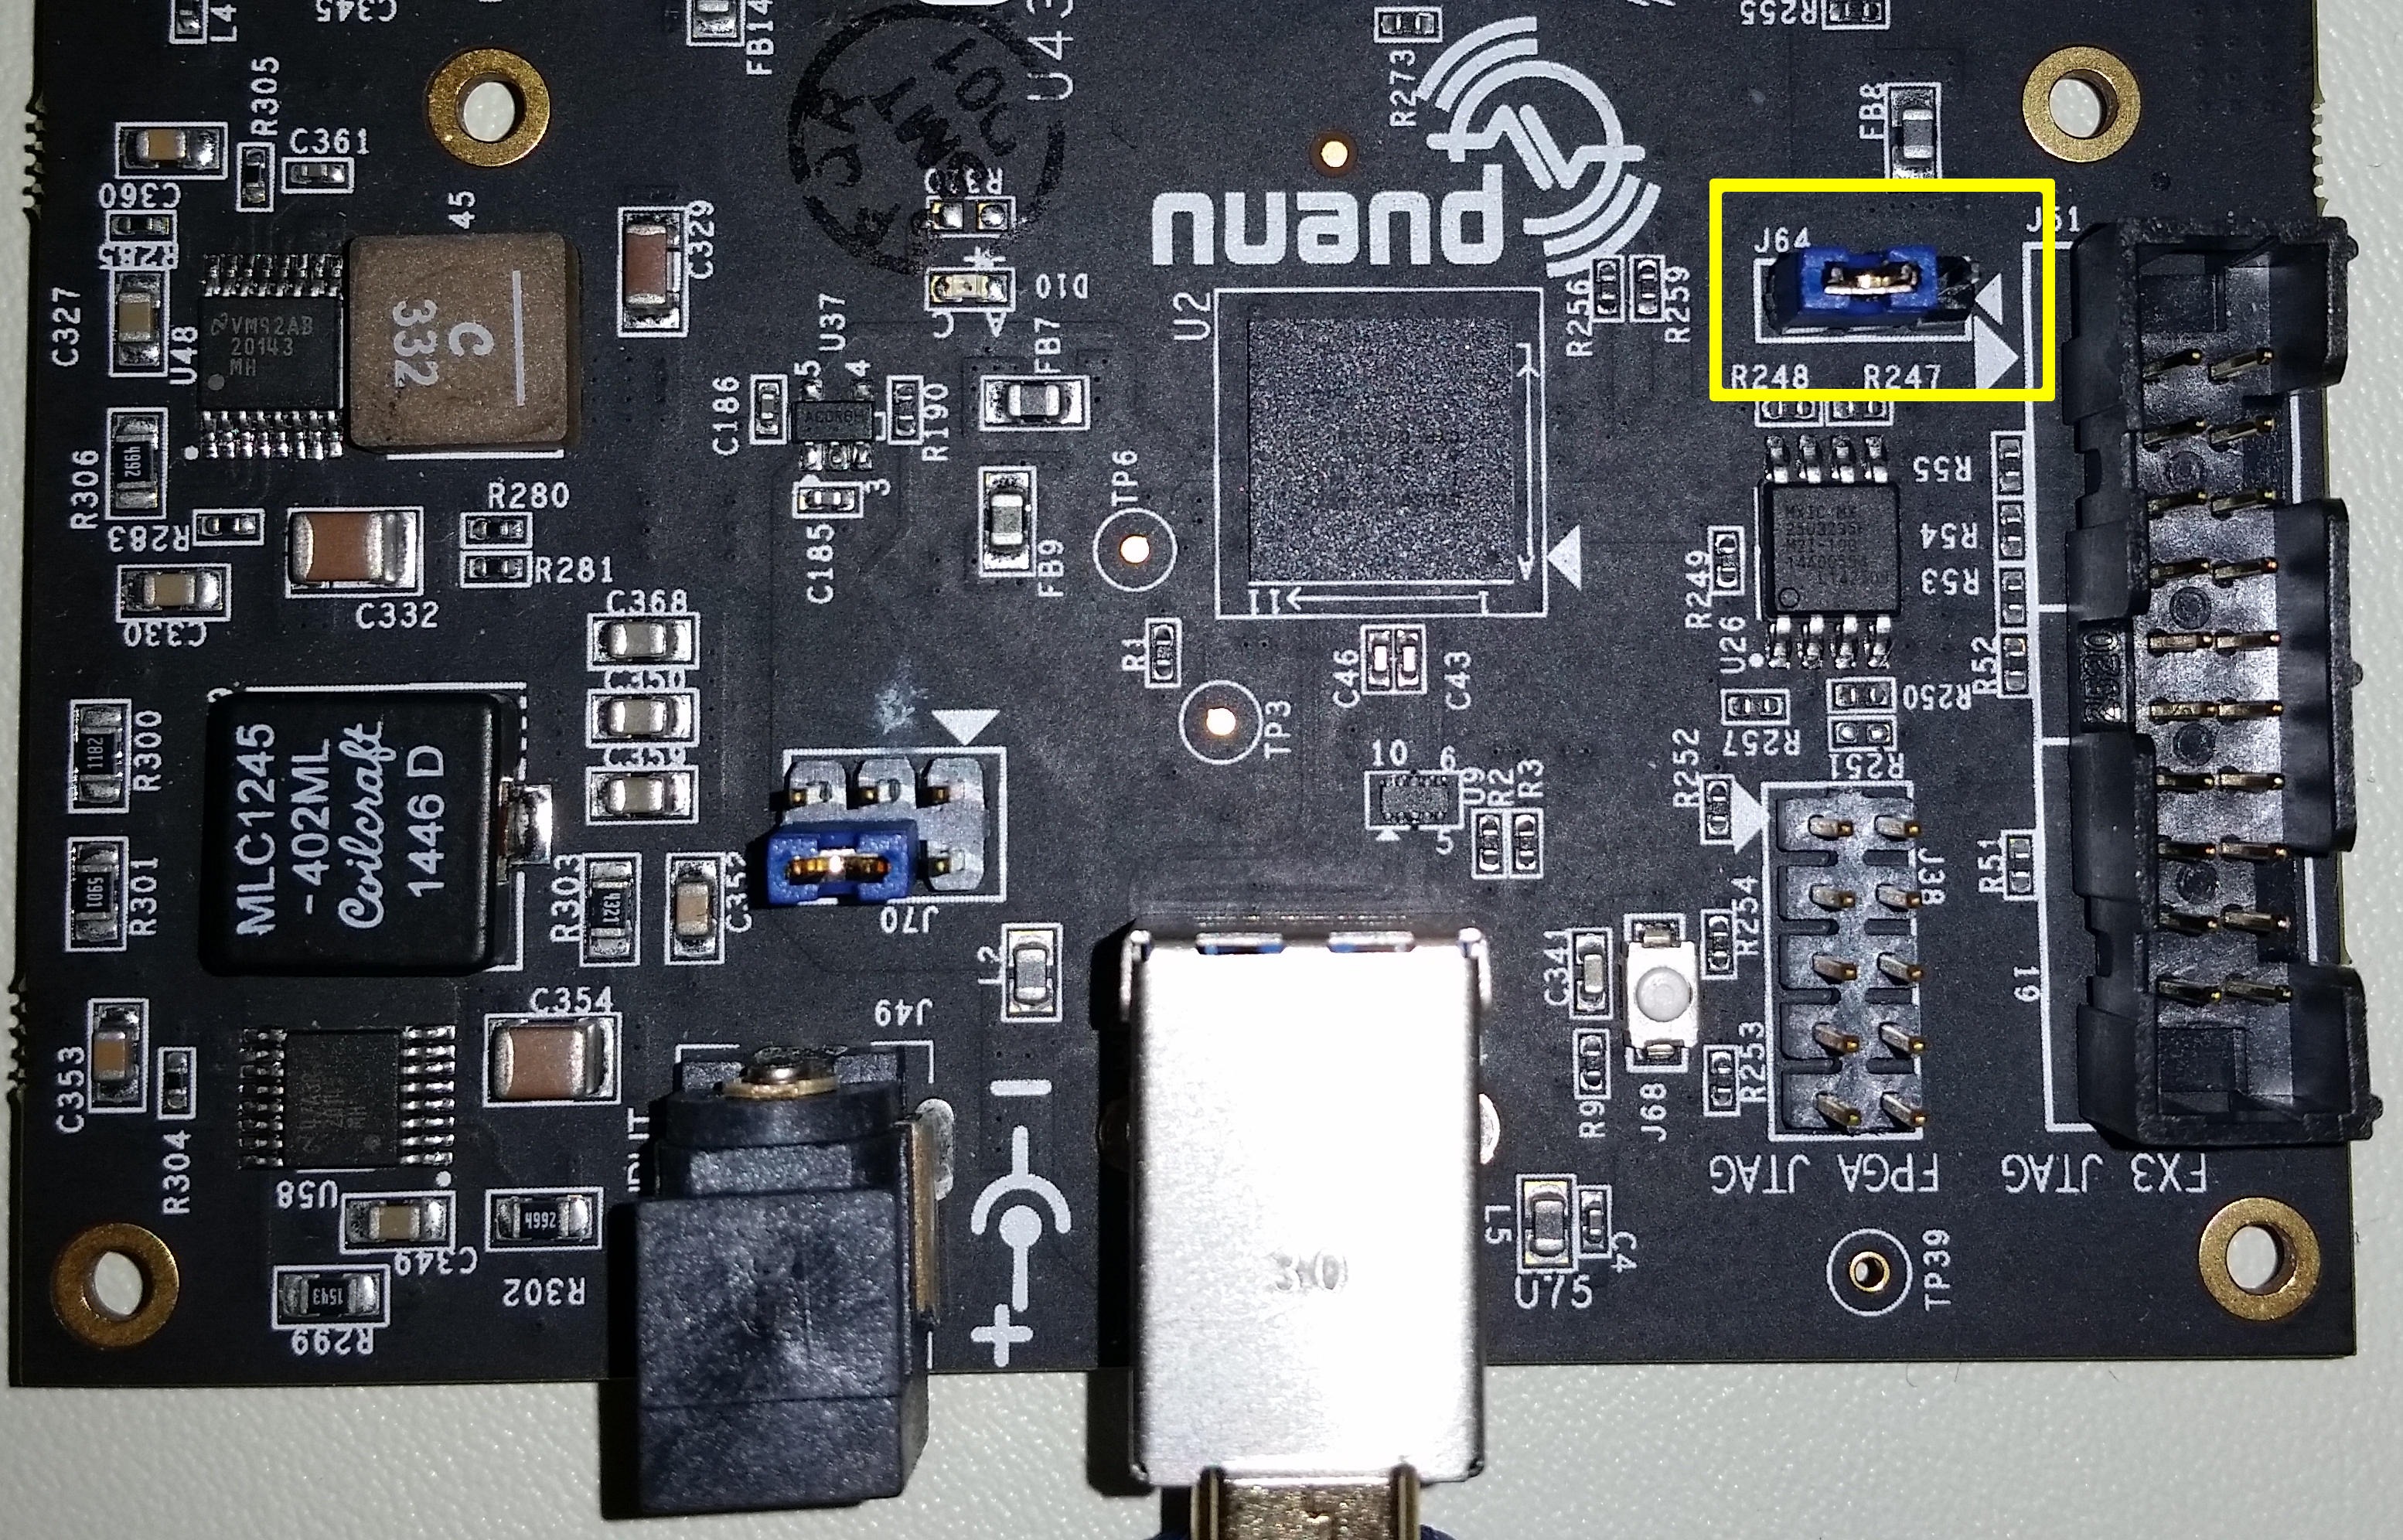
\includegraphics[width=4.5in]{images/bladeRF/j64-jumpered.jpg}
  \caption{bladeRF J64 jumper setting to force bootloader mode}
\end{figure}


To force the device into bootloader mode and re-flash firmware:
\begin{enumerate}
    \item Begin with the bladerf powered off.
    \item Place a jumper across pins 2 and 3 of header \texttt{J64}.
    \item Plug the device in to power it on.
    \item \textbf{Important}: Remove the jumper from \texttt{J64}.
        \begin{itemize}
            \item Forgetting this step will prevent the device from booting firmware in later steps.
        \end{itemize}
    \item Follow Section \ref{sec:recovery} to recover from the bootloader state
\end{enumerate}
